\begin{figure}[!htb]
\centering
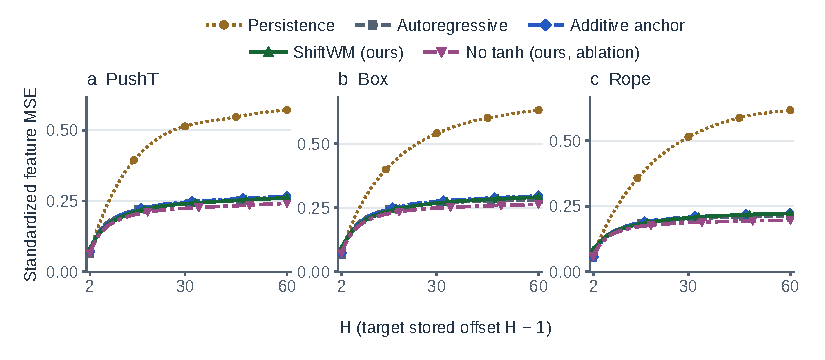
\includegraphics[width=\linewidth]{generated/iws_variant_forecasts/forecast_transfer_all_variants.pdf}
\caption[Complete IWS development forecasts and bound ablation.]{\textbf{Complete IWS development forecasts and the innovation-bound ablation.} All five predictors retain all 59 future offsets from one observed image; learned methods receive supplied causal command prefixes, while persistence ignores commands. The horizontal axis is $H=2,\ldots,60$, targeting stored offset $H-1$, not physical time. Training-standardized feature MSE weights windows within trajectory, trajectories and three seeds equally; lower is better. Each task has its own zero-based vertical scale. The no-$\tanh$ predictor removes only the correction bound and belongs to a separately registered exploratory follow-up after v1 development. All nine new and 27 original runs must pass finalization before this figure appears. No uncertainty bands are inferred; paired endpoint gains and intervals are in Table~\ref{tab:iws-unbounded-component}. Reserved upstream-validation data remain excluded.}
\label{fig:iws-forecast-transfer}
\end{figure}
